\documentclass[mathserif]{beamer}

\usetheme{Berkeley}
\usecolortheme{orchid}

\usepackage[utf8x]{inputenc}
\usepackage[english, russian]{babel}
\usepackage{color}
\usepackage{graphicx}
\graphicspath{ {../Images/} }

\title{Поиск семейств оптимальных маршрутов на морских картах}
\author{Иван Громаковский \\
Научный руководитель: А. С. Ковалев}
\institute{Санкт-Петербургский национальный исследовательский университет \\ информационных технологий, механики и оптики}
\date{13 мая 2015}

\begin{document}

\frame{\titlepage}
\note{Здравствуйте!}

\begin{frame}{Цели работы}
    \begin{itemize}[<+->]
        \item Формализация понятия оптимальности
        \item Поиск семейств оптимальных маршрутов для принятия
          решения пользователем
        \item Реализация алгоритма, работающая в режиме реального времени
    \end{itemize}
\end{frame}
\note {
1. И так понятно.
2. Надо что-то придумать тут.
3. Меньше секунды на запрос.
}

\begin{frame}{Актуальность задачи}
    Проблемы поиска единственного маршрута:
    \begin{itemize}[<+->]
        \item критерии оптимальности не всегда очевидны и формализуемы
        \item не оставляет выбора пользователю
        \item приводит к повышенной загруженности
    \end{itemize}
\end{frame}
\note {
1. Кратчайший путь не всегда самый лучший. Например, где-то может быть
платный проезд, также нужно учитывать глубину, загруженность. Также у
капитана могут быть личные предпочтения, которые невозможно
формализовать.
2. Зачастую пользователь хочет иметь возможность самостоятельно
выбрать маршрут.
3. Если приложение набирает популярность и все пользуются одинаковыми
(например, кратчайшими) маршрутами, это может приводить повышенной загруженности.

TODO: возможно, что-то ещё можно упомянуть?
}
        
\begin{frame}{Оптимальность маршрутов}
    Назовём семейством оптимальных маршрутов из одной точки в другую 
    максимальное по включению множество путей между этими точками,
    обладающее следующими свойствами:
    \begin{itemize}[<+->]
        \item для любых двух маршрутов найдётся препятствие, размеры
          которого сопоставимы с длиной кратчайшего из маршрутов,
          которое обходится с разных сторон
        \item TODO: получше сформулировать первый пункт
        \item TODO: ещё пункты?
    \end{itemize}
\end{frame}
\note{Слайд не готов}

\begin{frame}{Существующие алгоритмы}
    \only<1-3>{Известные алгоритмы множественного поиска путей в графе
      имеют следующие недостатки:}
    \begin{itemize}
        \item<1-3> разрабатывались для других целей
        \item<2-3> не учитывают топологию
        \item<3-3> строят очень похожие маршруты на морских картах
    \end{itemize}
    \only<4-4> {
        \begin{figure}
            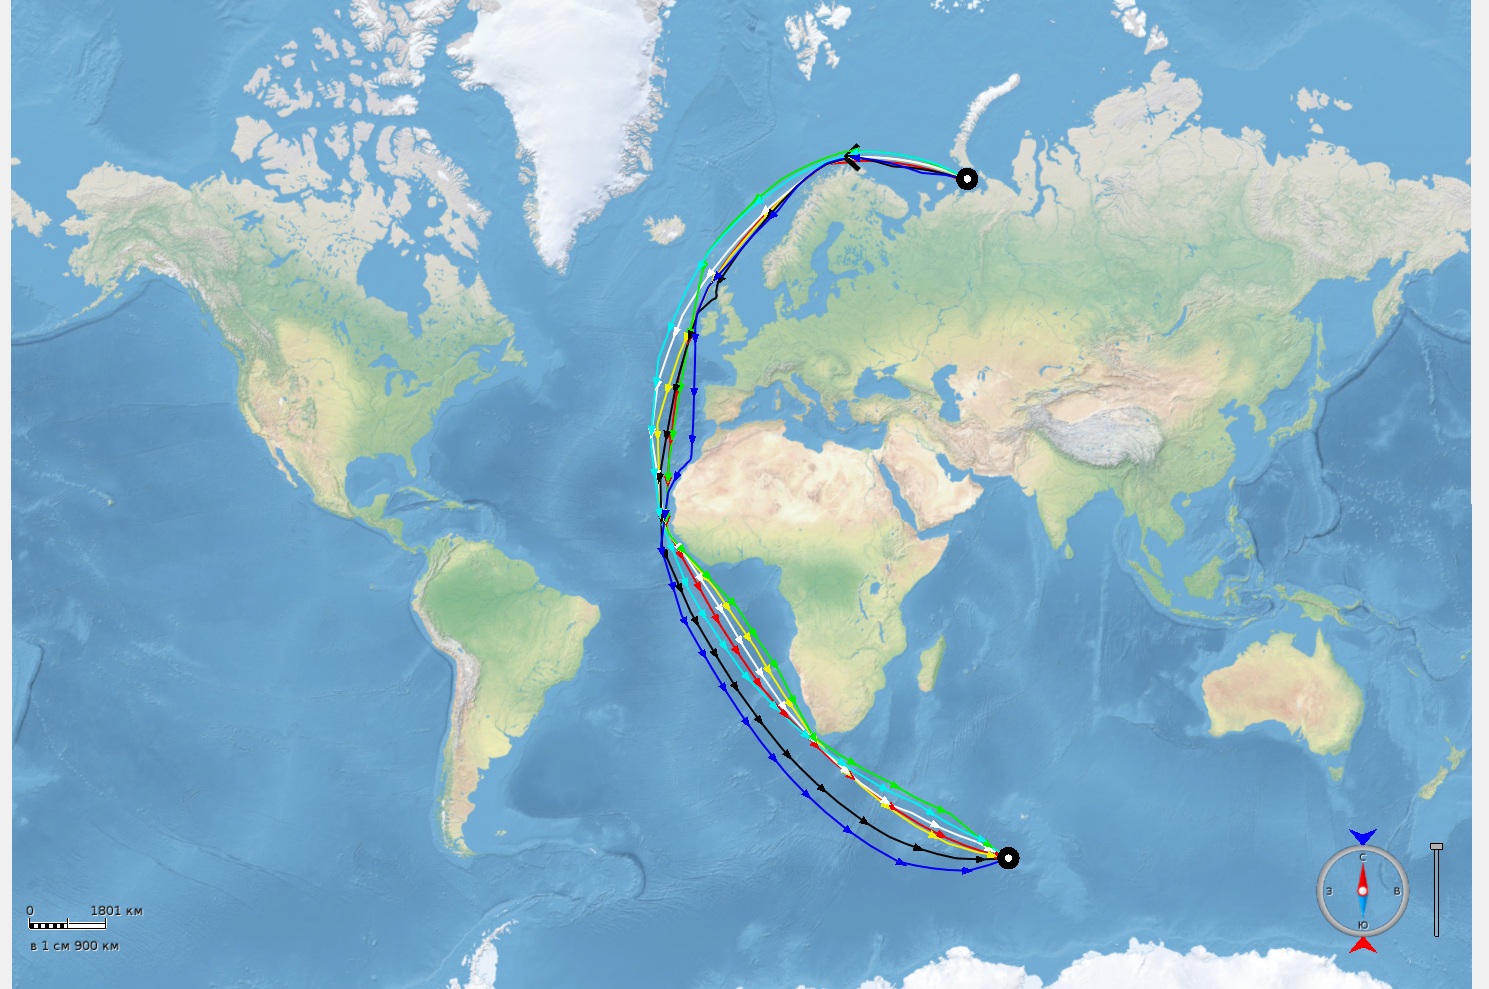
\includegraphics[width=\textwidth]{comparison-with-existing-bad}
            \caption{Результат работы существующего алгоритма}
        \end{figure}
    }
    \only<5-5> {
        \begin{figure}
            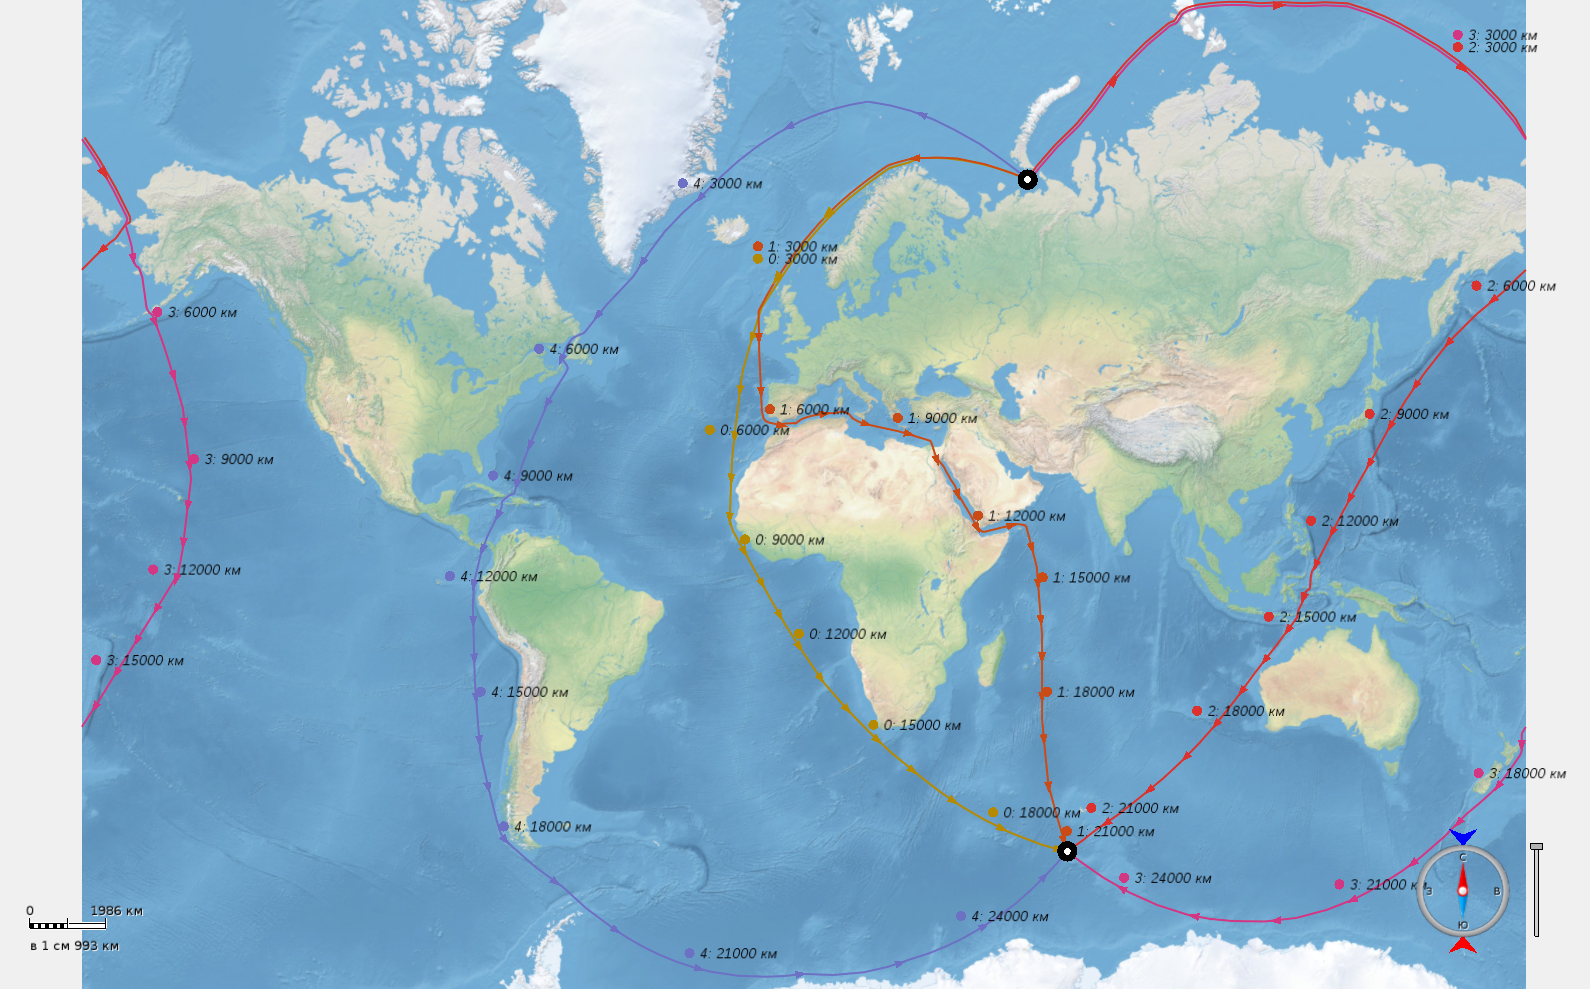
\includegraphics[width=\textwidth]{comparison-with-existing-good}
            \caption{Желаемый результат}
        \end{figure}
    }
\end{frame}

\begin{frame}{Предобработка данных}
    \begin{itemize}[<+->]
        \item Карта → полигон
        \item Оффсет (TODO: по-русски — смещение?) полигона
        \item Граф по сетке на плоскости + граф локальной видимости
        \item Ограничение длины ребра
        \item Дополнительные рёбра
    \end{itemize}
\end{frame}
\note {
1. Склеивание, упрощение. Полигон — множество контуров (в том числе дырок).
2. Корабли не плавают слишком близко к суше. Используется straight skeleton.
3. Чтобы находить кратчайший путь, нужен граф видимости. Но в нём
слишком много рёбер, поэтому построим навигационный граф. Разложим
вершины по сетке, проведём рёбра до соседей (и их соседей). Также
добавим вершины полигона и проведём из них рёбра до ближайших видимых 
вершин. Веса рёбер — расстояния между точками на сфере.
4. Путь ищется на сфере, при этом проверка корректности рёбер
осуществляется на плоскости. Кратчайшая траектория на сфере отличается
от кратчайшей траектории на плоскости. Не будем допускать слишком
длинные рёбра, тогда расхождение будет пренебрежимо мало.
5. Во-первых, добавим рёбра из straight skeleton'а, получившиеся в
результате схлопывания. Во-вторых, нужна возможность добавления рёбер
в связи с неточностями исходной карты. В-третьих, рёбра через 180-ый меридиан.
}

\begin{frame}{Поиск одного маршрута}
    \begin{itemize}
        \item<1-> Добавление вершин в граф
        \item<2-> Алгоритм Дейкстры
        \item<3-> Сокращение маршрута
        \begin{itemize}
            \item<3-> Если подпуть A → B → C можно выгодно заменить на A → C, заменяем 
            \item<3-> Подразбиение маршрута
        \end{itemize}
        \item<4-> Сглаживание маршрута
        \item TODO: картинка (картинки) для демонстрации
    \end{itemize}
\end{frame}

\begin{frame}{Поиск нескольких маршрутов}
    \begin{itemize}
        \item Поиск одного маршрута
        \item Обновление весов:
        \begin{itemize}
            \item Потенциалы как функция кратчайших расстояний от фиктивной вершины 
            \item Обновление потенциалов
            \item Применение потенциалов
        \end{itemize}
        \item Проверка критерия остановки:
        \begin{itemize}
            \item Длина маршрута
            \item Метрики на маршрутах
        \end{itemize}
    \end{itemize}
\end{frame}

\begin{frame}
    \frametitle{Обновление весов}
    \begin{itemize}
        \item Потенциалы должны быть множителями, а не слагаемымми
        \item TODO: Картинка
        \item На маршруте потенциалы меньше, чем поблизости
        \item TODO: Картинка
    \end{itemize}
\end{frame}

\begin{frame}
    \frametitle{Метрики}
    \begin{itemize}
        \item $\rho_1 (P, Q) = max_{u \in P} min_{v \in Q} \rho_g(u, v)$
        \item TODO: картинка для демонстрации
        \item TODO: вторая метрика
        \item TODO: картинка для демонстрации
    \end{itemize}
\end{frame}

\begin{frame}
    \frametitle{Вычисление метрик}
    \begin{itemize}
        \item Фиктивная вершина
        \item Обход Дейкстры, пока не посещены вершины второго пути 
        \item Заканчиваем, если достигли необходимого значения
        \item Поиск ближайшей вершины (вторая метрика) — перебором
        \item На практике затраты на вторую метрику такие же низкие
    \end{itemize}
\end{frame}

\begin{frame}
    \frametitle{Результаты}
    \begin{itemize}
        \item<1-1> Разработан и реализован алгоритм построения семейств оптимальных маршрутов 
        \item<1-1> Проведено сравнение с существующими подходами 
        \item<1-1> Поиск выполняется примерно за полсекунды 
    \end{itemize}
%    \putimg<2-2>{results.png}
\end{frame}

\end{document}

